%
% Auteur initial inconnu.
% Modifié par olivier.ploton@univ-tours.fr le 21/09/2021
% À compiler avec pdflatex, bibilographie avec biber.
% Tous les fichiers doivent être encodés en UTF-8
% S'utilise en présence du fichier de bibiographie biblio.bib
% et des dossiers polytech/ (classe) et pic/ (images)
%

\documentclass{polytech/polytech}
\usepackage[strings]{underscore} % utile pour les _ dans la biblio (DOI)

% Fixe la présentation des listings
\lstset{
 columns=fixed,       
 numbers=left,                              
 numberstyle=\tiny\color{gray},             
 frame=single,                              
 backgroundcolor=\color[RGB]{255,255,255},  
 keywordstyle=\color[RGB]{40,40,255},       
 numberstyle=\footnotesize\color{darkgray}, 
 commentstyle=\it\color[RGB]{0,96,96},      
 stringstyle=\rmfamily\slshape\color[RGB]{128,0,0},  
 showstringspaces=false,                    
 language=C++
}

% Quelques formatages supplémentaires
\numberwithin{figure}{chapter}
\renewcommand\thesubsection{\thesection.\arabic{subsection}} 

% dossier des images
\graphicspath{{./pic/}}

%%%%%%%%%%%%%%%%%%%%%%%%%%%%%%%%%%%%%%%%

%
% Paramètres à fixer avant de commencer le document
%

\typereport{prddi5}       

\reportyear{2023-2024}

\title{Optimisation des déplacements d’échantillons médicaux dans le cadre de la Sclérose Latérale Amyotrophique
(SLA ou Maladie de Charcot)}

\reportlogo{polytech/polytech}
           
\student[di5]{Florian}{BETHENCOURT}{florian.bethencourt@univ-tours.fr}

\academicsupervisor[di]{Jean-Charles}{BILLAUT}{jean-charles.billaut@univ-tours.fr}

\resume{%
Ce projet vise à développer un modèle mathématique permettant d'optimiser le transport d'échantillons médicaux de patients atteints de la SLA. À termes l'outil développé sera capable de prendre des données de centres d'analyse en entrée et de fournir en sortie une solution optimale et un ensemble d'instructions à suivre pour chacun des centres d'analyse pour mettre en place cette solution optimale.\\
Ce rapport introduit le sujet, présente un état de l'art sur les recherches similaires et décrit tout l'avancement du projet pour le semestre 9, de l'analyse du problème au début du développement du modèle.
Il contient également le planning prévu initialement et le vrai planning suivi, ainsi que les fonctionnalités du système.
}

\motcle{Contraintes}
\motcle{Échantillons médicaux}
\motcle{Flots}
\motcle{Graphe}
\motcle{Maladie de Charcot}

             
\abstract{
This project aims to develop a mathematical model for optimizing the transportation of medical samples from patients with ALS. Ultimately, the developed tool will be capable of taking input data from analysis centers and providing an optimal solution as output, along with a set of instructions for each analysis center to implement this optimal solution.\\
This report introduces the topic, presents a state-of-the-art overview of similar research, and describes the progress of the project for semester 9, from problem analysis to the early stages of model development. It also includes the initially planned schedule, the actual schedule followed, and the system's functionalities.
}
\keyword{Constraints}
\keyword{Medical samples}
\keyword{Flows}
\keyword{Graph}
\keyword{Lou Gehrig's disease}

%
% Le poster. Il faut exactement 3 blocs.
%

\posterblock{Objectifs}{
Le transport d'échantillons médicaux entre différents centres d'analyses éparpillés sur le territoire est un problème complexe à résoudre et extrêmement utile pour beaucoup de recherches médicales. Ce projet vise à développer un modèle mathématique capable d'optimiser la répartition des échantillons dans le cadre de la maladie de Charcot.
}{pic/graph1.png}{}

\posterblock{Mise en œuvre}{
Pour cela le modèle doit répondre à tout un ensemble de contraintes spécifiques à la conservation des échantillons sanguins tout en limitant la distance qu'ils parcourent et leur temps de trajet. Une fois perfectionnée, le modèle devra être implémenté sur un solveur mathématique.
}{pic/graph2.png}{}

\posterblock{Résultats attendus}{
On attend une solution approchée voire optimale du problème avec un tableau contenant l'ensemble du flux des échantillons entre les différentes villes ainsi qu'un ensemble d'instructions à suivre pour appliquer cette solution.
}{pic/graph3.png}{}


\newglossaryentry{graphe}
{
	name=Graphe,
	description={On appelle graphe un ensemble de points appelés sommets couplé à un ensemble de lignes appelées arêtes ou arcs qui relient certains sommets entre eux.}
}

\newglossaryentry{aliquotage}
{
	name=aliquotage,
	description={L'aliquotage est une opération consistant à séparer un tube en plusieurs tubes de quantité plus faible.}
}

\newglossaryentry{heuristiques}
{
	name=heuristiques,
	description={Une heuristique est une méthode de calcul qui fournit rapidement une solution réalisable, pas nécessairement optimale ou exacte, pour un problème d'optimisation difficile.}
}


\newacronym{sla}{SLA}{Sclérose Latérale Amyotrophique, aussi appelée Maladie de Charcot.}
\newacronym{vrp}{VRP}{Vehicle Routing Problem, ou Problème de Tournée de Véhicules en français.}
\newacronym{tsp}{TSP}{Travelling Salesman Problem, ou Problème du Voyageur de Commerce en français.}

\bibliography{biblio}
\makeglossaries

%%%%%%%%%%%%%%%%%%%%%%%%%%%%%%%%%%%%%%%%

\begin{document}
             
\chapter{Introduction}
\section{Acteurs, enjeux et contexte}

Présentation du contexte des acteurs et des enjeux.

Acteurs:
\begin{itemize}
\item Client : BLASCO Hélène
\item MOA : BILLAUT Jean-Charles
\item Auteur : BETHENCOURT Florian\\
\end{itemize}

\begin{flushleft}
La Sclérose Latérale Amyotrophique (SLA) ou maladie de Charcot est une maladie du neurone moteur qui se caractérise par une perte progressive des neurones moteurs du cerveau et de la moelle.  Le projet se focalise sur un consortium constitué de cinq centres hospitaliers qui se sont spécialisés dans l’étude de cette maladie.\\
Deux centres en France disposent d’une grande cohorte de patients : Lille (L) et Tours (T). Ces centres prélèvent notamment sur les patients du sang, du liquide céphalo-rachidien (LCR) et du plasma, et les stockent selon différentes conditions de conservation (température, tubes/poches, volumes, etc.). Trois autres centres, spécialisés dans cette maladie, s’ajoutent au consortium pour les explorations biologiques : Lyon (Ly), Montpellier (M) et Poitiers (P).\\
Afin de consolider les résultats des analyses, il est important que ces centres travaillent sur les échantillons en provenance des mêmes patients, ce qui nous amène à notre problème.
\end{flushleft}

\begin{flushleft}
L’objectif de ce projet est de proposer le parcours optimal des échantillons des différentes
cohortes afin d’éviter la perte et la dégradation des paramètres biologiques. À terme, ce projet pourra même
se généraliser à des études cliniques concernant d’autres maladies, pour d’autres types de
prélèvements et d’analyses, et pourra concerner d’autres centres hospitaliers.\\
Pour faire cela, on va modéliser le problème sous la forme d’un programme linéaire en nombres entiers, puis on étudiera sa résolution par des solvers du marché. Dans la suite du rapport, nous utiliserons des graphes à la fois pour imager le flux d'échantillons entre les 5 villes, ainsi qu'à l'intérieur même du modèle mathématique pour représenter au mieux les contraintes réelles.
\end{flushleft}


\section{Objectifs}
L'objectif final de ce projet est de proposer un algorithme (approché et/ou exact) aux différents centres d'analyses pour organiser au mieux la répartition, le transport et l'analyse des échantillons.\\

Le premier objectif est d'implémenter un modèle intégrant le plus possible de contraintes liées à la répartition des échantillons sanguins, à savoir : 
\begin{itemize}
    \item Contrainte de congélation : Afin de préserver au maximum l'intégrité des échantillons, ceux-ci sont congelés lors du transport (à -80°C ou -20°C) et décongelés lors des analyses. Chaque cycle de congélation/décongélation (appelé cycle C/D par la suite) détériore l'échantillon, il faut donc les limiter au maximum. De plus certaines analyses requiert le même nombre de cycle C/D pour tous les échantillons.
    \item Contrainte d'aliquotage : L'\gls{aliquotage} est une opération consistant à séparer un tube en plusieurs tubes de quantité plus faible. Cependant c'est une opération fastidieuse et source d'erreurs, il faut donc essayer de minimiser son utilisation
    \item Contraintes liées au flux : Ce sont des contraintes évidentes mais obligatoires et nécessaires au bon fonctionnement du modèle. Une ville ne peut pas envoyer plus que ce qu'elle reçoit, les quantités envoyées ne peuvent pas dépasser la capacité max d'un tube, ect...\\
\end{itemize}

\begin{flushleft}
Ce sont les contraintes principales, mais en fonction de l'avancée du projet on pourra en ajouter d'autres pour coller toujours mieux à la réalité (en fonction bien sûr de leur faisabilité). Par exemple, il faudrait que les échantillons provenant de Lille et ceux provenant de Tours soient mélangés pendant les analyses.
\end{flushleft}

\begin{flushleft}
Le 2ème objectif principal est d'implémenter le modèle sur un solveur mathématique afin de pouvoir l'analyser. Cela permettra en premier lieu d'avoir un aperçu des performances et de la pertinence du modèle notamment lors de la mise à l'échelle, et de le modifier en fonction des résultats obtenus. Dans un second temps on pourra se servir de ces résultats pour rédiger la marche à suivre par chacun des centres hospitaliers.
\end{flushleft}

\begin{flushleft}
Le 3ème et dernier objectif principal est de développer un outil d'aide multicritère à la décision qui optimise le flux de ces échantillons, tout en respectant les contraintes imposées.
Cette dernière partie ne sera pas abordée pour cette année, mais fera l'étude d'un autre PRD suivant celui-ci.
On se focalisera plutôt sur une modélisation fonctionnelle du problème, ainsi qu'une documentation complète et compréhensible de son implémentation afin de faciliter au mieux la reprise de ce sujet.  
\end{flushleft}

\section{Hypothèses}

À partir d'un certain nombre de contraintes et surtout lors de la mise à l'échelle, le modèle créé sur Gusek ne pourra plus être solvable en temps acceptable.\\
Il faudra donc passer sur un solveur mathématique, mais cela signifie qu'on ne pourra plus tester la faisabilité du modèle à l'avance, et par conséquent qu'il faudra modifier les contraintes "à l'aveugle". Ainsi il sera préférable de complexifier au maximum le modèle sur Gusek avant de l'implémenter.
\pagebreak

\section{Bases méthodologiques}
\begin{itemize}
\item Les outils : 
\begin{itemize}
    \item Pour la gestion de projet, on utilisera le diagramme de Gantt pour contrôler le déroulement du projet.
    \item Pour la modélisation du modèle, on utilisera « Gusek ». Le solveur mathématique n'a pas encore été fixé mais on utilisera probablement « Cplex ».
    \item Pour la rédaction du rapport, on utilisera « LaTex ».\\
\end{itemize}

\item La méthode de gestion de projet :\\
On utilise le modèle en « cascade » (Figure1.1) pour gérer ce projet. Chaque tâche s'effectue dans l'ordre, de haut en bas et nécessite d'avoir complété la tâche précédente.
Les attendus et la définition du projet étant bien fixées, ce modèle convient parfaitement.\\
\begin{figure*}[h!]
    \centering 
    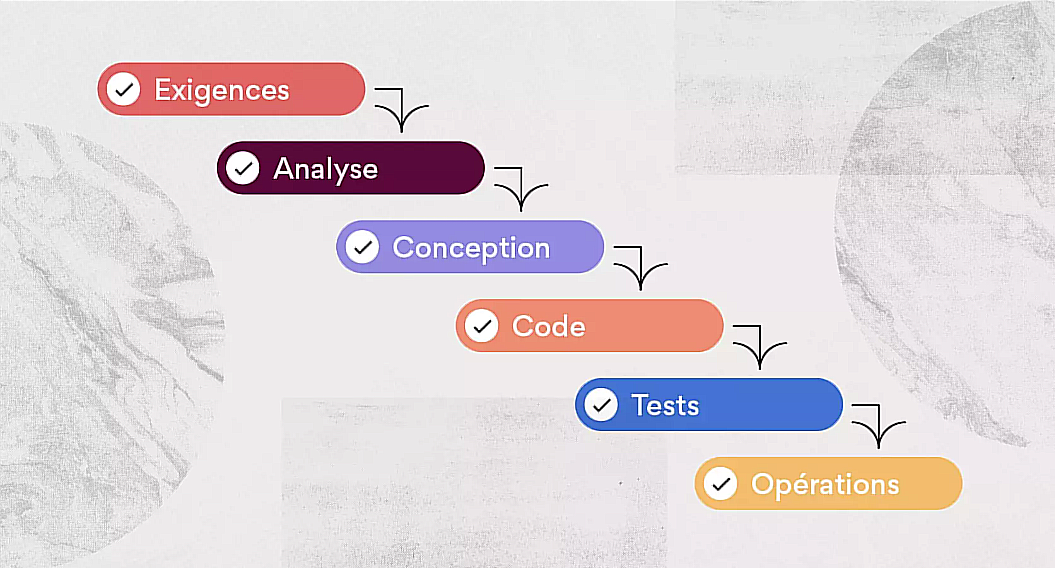
\includegraphics[width=0.9\textwidth]{pic/cascade.png} 
    \caption{Modèle en cascade}
    \label{Modèle en cascade}
\end{figure*}

Pour le semestre 9, on nous demande de nous concentrer sur la prise en main du sujet et la définition précise du travail à affectuer. Cela correspond aux tâches d'Exigences et d’Analyse.
J'ai cependant déjà pu m'avancer sur la partie Conception comme nous le verrons dans la suite du rapport.
\end{itemize}

\chapter{Description générale}
\section{Environnement du projet}

L’environnement de développement est le suivant :
\begin{itemize}
    \item Le système d’exploitation : Windows;
    \item Le logiciel de modélisation : Gusek;
    \item Le matériel pour le développement : Machine personnelle ou PC fixe de Polytech\\
\end{itemize}

Les différents acteurs du projet peuvent également être amenés à faire des réunions en présentiel ou visio par Teams pour discuter des contraintes à rajouter ou modifier, ou simplement s'échanger des mails.


\section{Caractéristiques des utilisateurs}

Seul l'étudiant ou l'encadrant sera amené à utiliser le logiciel tel quel, étant donné que son utilisation nécessite une connaissance approfondie du sujet et de l'informatique. Cependant les résultats obtenus seront des instructions à suivre et/ou des propositions d'organisation des échantillons à évaluer par le personnel des centres d'examen.
\pagebreak

\section{Fonctionnalités du système}
Les fonctionnalités du système sont plutôt simples : \\

\begin{figure}[h]
    \centering
    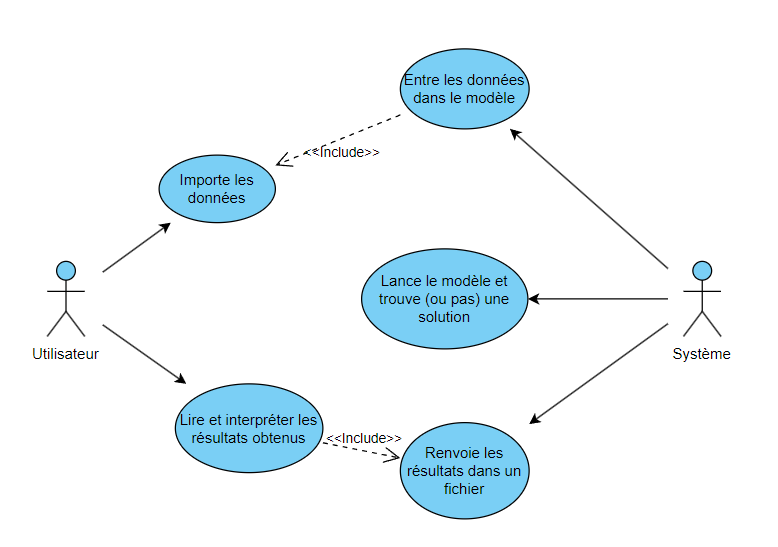
\includegraphics[width=0.9\textwidth]{pic/usecase.png}
    \caption{Diagramme de cas d'utilisation}
    \label{fig:use_case1}
\end{figure}

En pratique, les données d'entrée vont très peu changer : elles correspondent aux villes d'études (5 dans notre cas), et aux quantités produites et demandées d'échantillons de différents types pour chaque ville.

Si le système trouve une solution, les résultats envoyés seront les flux d'échantillons pour chaque ville, regroupés dans un grand tableau. On peut ensuite se servir de ces données pour imager le flux à réaliser et rédiger en conséquence la marche à suivre pour tous les centres d'analyse.

La partie Modélisation mathématique rentre plus en détail dans le fonctionnement du modèle implémenté.

\section{Structure générale du système}

Il n'y a que 4 composantes dans le systèmes, à savoir : 
\begin{itemize}
    \item Le modèle construit sur Gusek
    \item Son implémentation sur le solveur mathématique
    \item Un ou plusieurs fichiers de données d'entrée
    \item Un ou plusieurs fichiers de sortie contenant les résultats du solveur
\end{itemize}

\chapter{État de l'art / Veille technologique}

À notre connaissance, le problème n'a pas été abordé sous cet angle dans la recherche. Cependant il existe de nombreux articles concernant des problèmes similaires, que nous allons aborder ici.

\section{Voyageur de commerce et tournée de véhicule}

Le problème du voyageur de commerce (TSP en anglais pour Travelling Salesman Problem) est un problème très connu en informatique, et les algorithmes permettant sa résolution sont très documentés. Le problème de la tournée de véhicule (VRP en anglais pour Vehicle Routing Problem) est un dérivé du 1er, et les deux se présentent ainsi : 

\begin{figure*}[h]
    \centering
    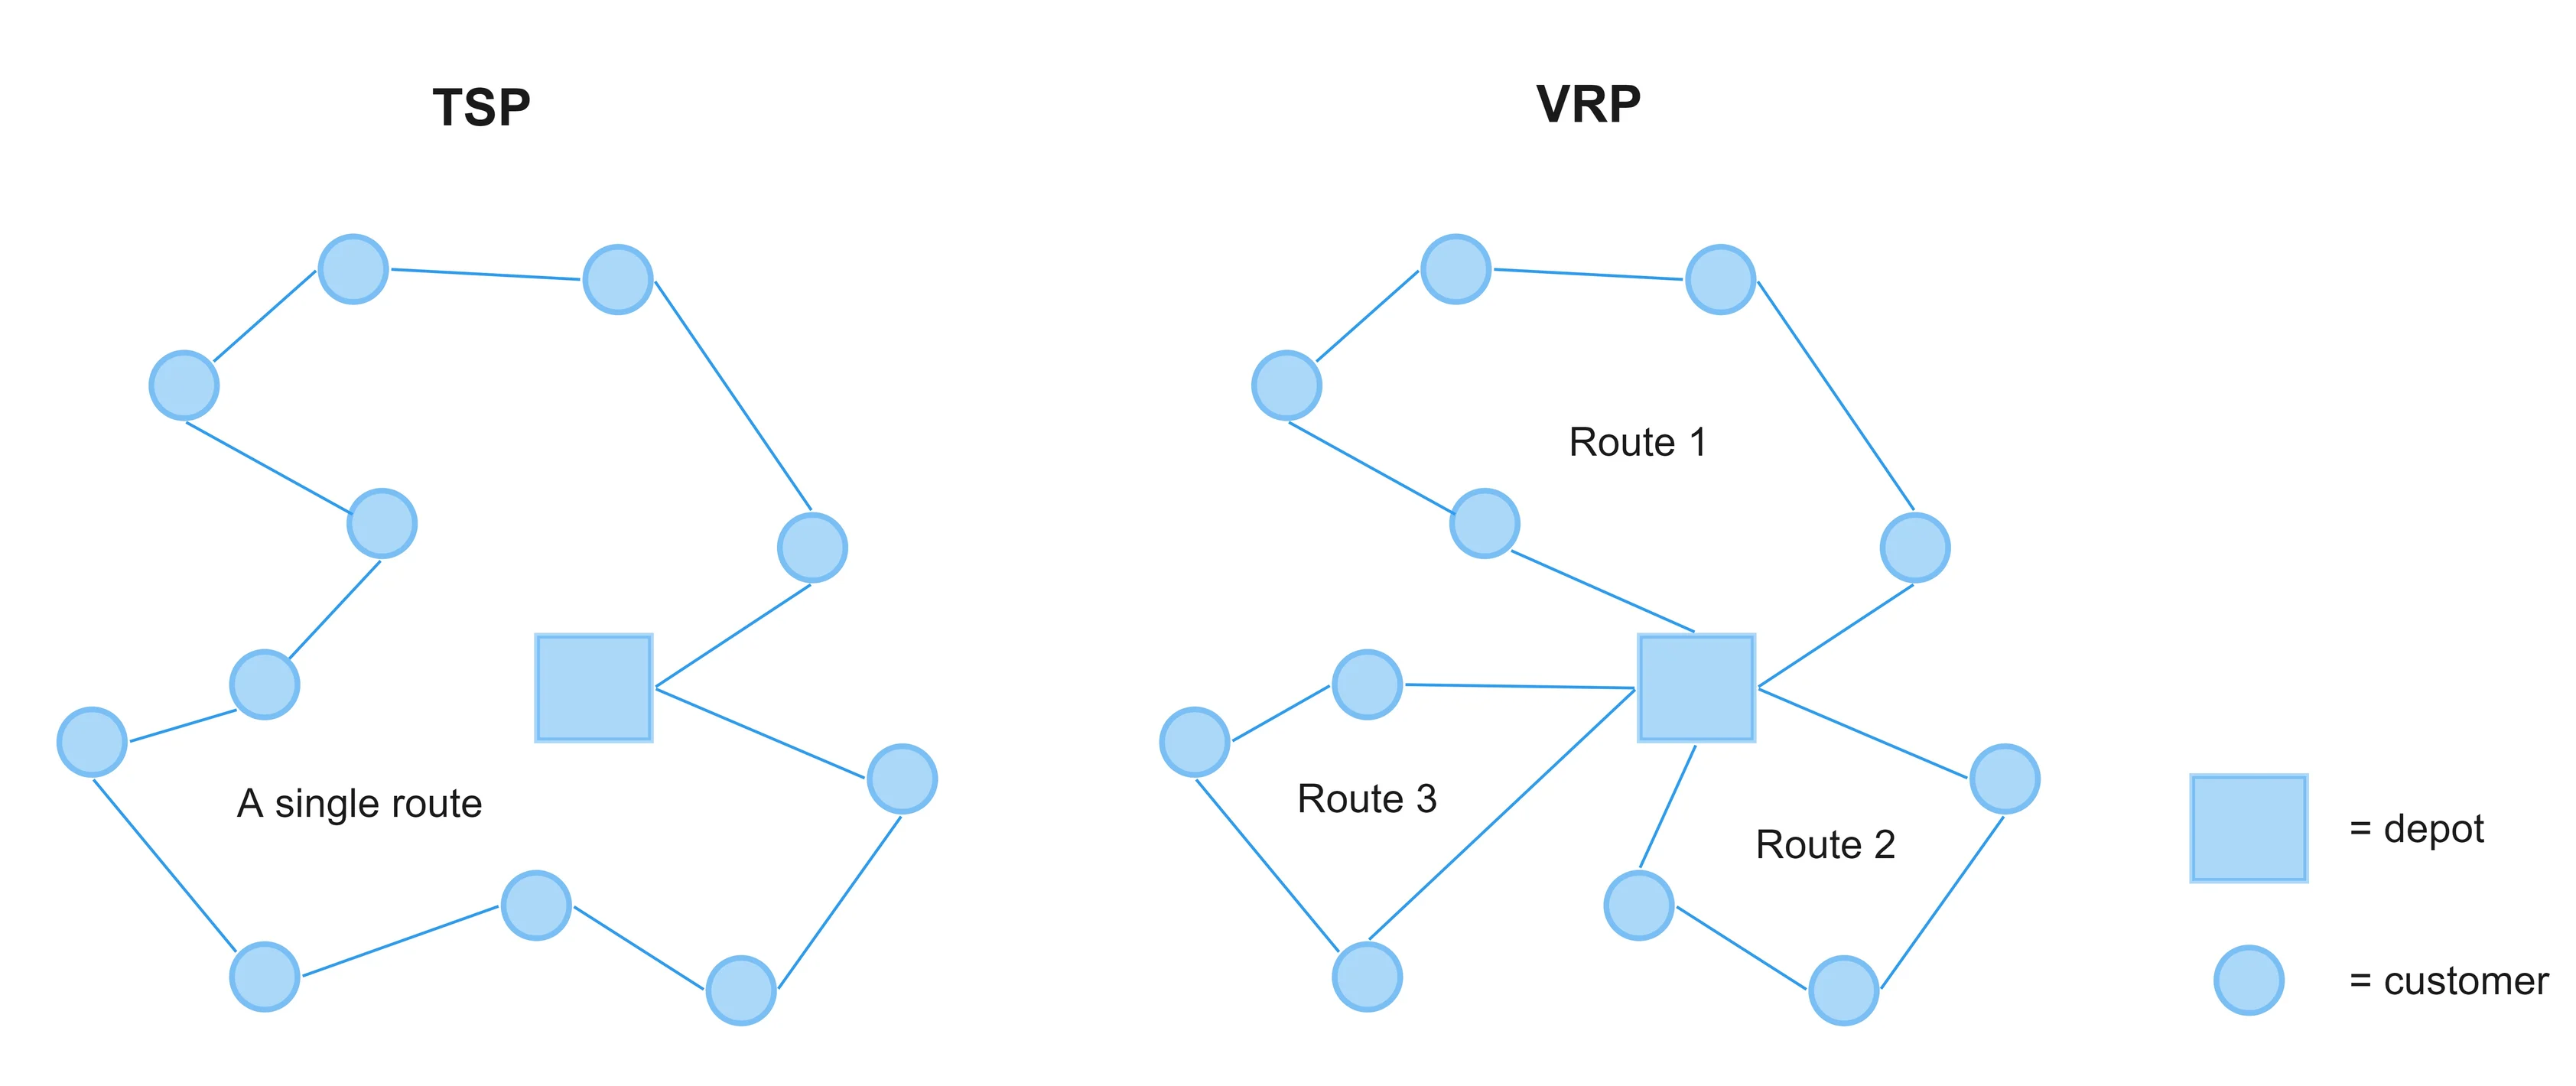
\includegraphics[width=0.9\textwidth]{pic/TSPVRP.png}
    \caption{Illustration DU TSP et VRP}
    \label{Illustration DU TSP et VRP}
\end{figure*}

Le TSP considère un ensemble de villes, où le but est de passer une seule et unique fois par chacune d'entre elles et de revenir au point de départ, en minimisant au maximum la distance du trajet parcouru.\\
Le VRP étend le problème à un ensemble de trajets et de véhicules, où l'objectif est d'affecter à chaque ressource un trajet permettant de couvrir l'ensemble des villes à traverser, tout en répartissant la charge de façon équitable entre toutes les ressources. 

Par exemple dans ce papier \cite{VRP}, les 3 chercheurs se focalisent sur la résolution d'un VRP où les "clients" sont des centres de collecte du sang et où le "dépôt" est le centre d'analyse. Ils utilisent pour cela différentes \gls{heuristiques} et les comparent entre elles, le but étant de trouver le nombre optimal de camions pour assurer au mieux la collecte et le transport des échantillons en respectant différentes contraintes de temps, d'argent et de conservation des échantillons sanguins.

Notre sujet prend en quelque sorte le problème du VRP à l'envers : Au lieu d'aller du client au dépôt comme dans la plupart des études concernant le transport d'échantillons de sang, on part du dépôt pour livrer tous les clients. Il conviendrait donc de replacer le môt "dépôt" par source qui fait plus de sens dans notre cas, ce qui nous donne un schéma comme cela : 

\begin{figure*}[h]
    \centering
    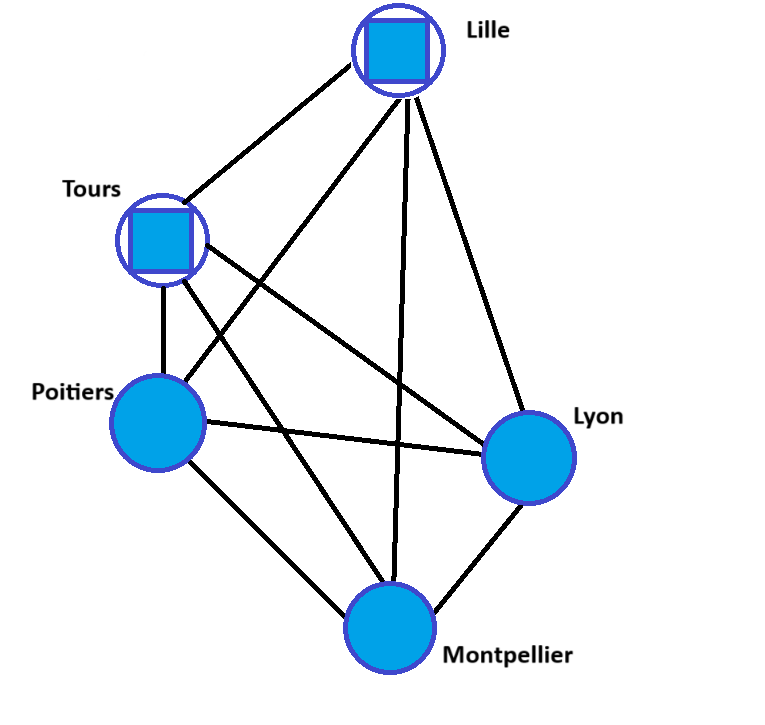
\includegraphics[width=0.9\textwidth]{pic/VRPPRD.png}
    \caption{Illustration du sujet sous la forme d'un VRP}
    \label{Illustration du sujet sous la forme d'un VRP}
\end{figure*}

On peut facilement mettre en lumière les différences entre les problèmes classiques de VRP et le nôtre : 
\begin{itemize}
	\item Comme dit plus haut on prend les routes "à l'envers".
	\item Il y a plusieurs sources, et une même route peut être empruntée par des échantillons provenant de sources différentes, ou au contraire utilisée par une seule source uniquement.
	\item L'échantillon n'a pas besoin de revenir au point de départ, puisqu'on considère que les cohortes se servent en premier avant de distribuer le reste des échantillons aux autres centres d'analyse.
\end{itemize}

Toutes ces raisons font que les méthodes de résolution classique du VRP ne peuvent pas s'appliquer à notre problème, ce qui implique de trouver de nouveaux algorithmes et méthodes de résolution.


\chapter{Analyse et conception}

\section{Analyse}

\subsection{Explication du graphe}
Afin de modéliser correctement le modèle de façon mathématique, on a décidé de le représenter sous forme d'un graphe, où les villes représentent les sommets et les arcs correspondent à l'envoi d'échantillons d'une ville à l'autre.

En plus des 5 villes, on ajoute également 3 sommets "fictifs" : 
\begin{itemize}
	\item S : C'est le sommet Source, qui va envoyer aux 2 cohortes (ici Tours et Lille) les quantités initiales de chaque tube.
	\item OK : C'est le sommet qui représente l'utilisation des échantillons par une ville.
	\item P : C'est le sommet Puits, qui va recevoir toutes les quantités en trop non utilisées\\
\end{itemize}

On peut alors obtenir un graphe comme celui-ci : \\

\begin{figure*}[ht]
    \centering
    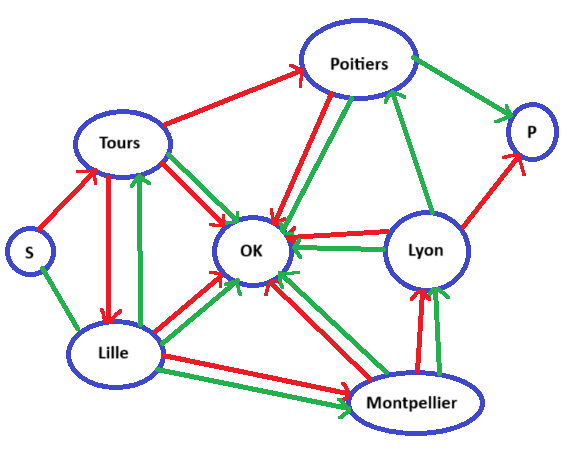
\includegraphics[width=0.9\textwidth]{pic/graph.png}
    \caption{Exemple de graphe possible}
    \label{Exemple de graphe possible}
\end{figure*}


\textcolor{red}{En rouge : Flux d'échantillons des patients de Tours}\\
\textcolor{green}{En vert : Flux d'échantillons des patients de Lille}\\

On aurait pu utiliser des arcs réflexifs (arc qui part d'un sommet et pointe vers le même sommet) pour dire qu'une ville utilise une partie des échantillons mais il était plus simple de faire ça avec un sommet bien distinct pour la création des contraintes du modèle (voir partie Modélisation mathématique).

\subsection{Contraintes imposées}
Le modèle à implémenter doit respecter un certain nombre de contraintes, fournies par Dr.BLASCO Hélène, vice-présidente de la recherche au CHRU de Tours.
Elles sont au nombre de 6 :
\begin{itemize}
	\item Tous les échantillons sont précieux, par conséquent il faut jeter le moins possible de sérum, plasma et liquide céphalo-rachidien.
	\item Prendre en compte le nombre de cycles congélation/décongélation de chaque tube et le minimiser. \\En effet les tubes doivent être congelés pour être transportés et décongelés pour pouvoir les analyser.
	\item Empêcher certaines analyses si tous les tubes n'ont pas le même nombre de cycle C/D.
	\item Limiter l'\gls{aliquotage} des tubes, car c'est une opération source d'erreurs.
	\item Intégrer une notion de temps aux analyses, car certaines sont plus longues que d'autres ou bien prioritaires.
	\item Enfin mixer des échantillons de Tours et de Lille dans les analyses afin qu'ils soient traités en même temps.\\

Ces contraintes sont susceptibles d'être modifiées en fonction des échanges avec Dr.BLASCO par rapport à l'avancée du modèle et des potentielles difficultés rencontrées.
\end{itemize}
\pagebreak

\section{Modélisation mathématique}

\subsection{Données}

\subsubsection{Données d'entrée constantes}

\begin{itemize}
	\item villes : Liste contenant les 5 villes : "Tours, Poitiers, Lyon, Lille, Montpellier".
	\item ville\_dep : Liste contenant les cohortes (ou villes de "départ") : "Tours, Lille".
	\item sp : Liste contenant les 3 sommets fictifs : "S, P, OK".
	\item typeTube : Liste contenant les 3 types d'échantillons : "PLA, SER, LCR" pour Plasma, Sérum et Liquide Céphalo-Rachidien.
	\item nbTubes : Tableau à 2 dimensions [ville\_dep, typeTube] d'entiers contenant le nombre de tubes d'un certain type prélevés par patient pour chaque cohorte.
	\item qtTubes : Tableau à 2 dimensions [ville\_dep, typeTube] de réels contenant la quantité prélevée d'un certain type de tube par patient pour chaque cohorte.
	\item demande : Tableau à 2 dimensions [villes, typeTube] de réels contenant les demandes en mL de chaque type de tube pour chacune des villes.
	\item HV : Réel arbitrairement grand nécessaire à l'écriture de certaines contraintes, strictement supérieure au flux maximum d'une ville à l'autre.
\end{itemize}

\subsubsection{Variables du modèle}

\begin{itemize}
	\item PhiT : Tableau à 4 dimensions [villes+sp, villes+sp, typeTube, nbTubes] de réels contenant la quantité envoyée d'un certain type de tube d'un patient de la cohorte de Tours d'une ville (ou sommet fictif) à une autre via un numéro de tube particulier.
Pour résumer, si on a PhiT["Tours", "Poitiers", "SER", "2"] = 0.2, cela signifie que Tours a envoyé à Poitiers 0.2mL de sérum via le tube n°2.
	\item PhiL : Même chose pour les patients de la cohorte de Lille.
	\item puits : Réel contenant la somme de tout ce qui a été jeté.
	\item congelT : tableau à 3 dimensions [villes, typeTube, nbTubes] de type booléen indiquant si le tube a subi un cycle C/D lors du départ de la ville.
	\item nbCongelT : tableau à 2 dimensions [typeTube, nbTubes] de réels comptant le nombre de congélations par tube.
	\item congelL : idem pour le flux de Lille.
	\item nbCongelL : idem pour le flux de Lille.
	\item envoiT : tableau à 4 dimensions [villes, villles, typeTube, nbTubes] de type booléen indiquant si une ville envoie quelque chose à une autre via un tube précis.
	\item aliT : tableau à 3 dimensions [villes, typeTube, nbTubes] d'entiers comptant le nombre d'aliquotages d'une ville pour un tube donné.
	\item envoiL : idem pour le flux de Lille.
	\item aliL : idem pour le flux de Lille.\\
\end{itemize}

Plutôt que d'utiliser 2 flux différents, on pourrait aussi pu rajouter une dimension de plus de taille ville\_dep. Cela est un choix arbitraire et il est tout à fait possible que l'on change la façon dont on définit le flux en fonction des contraintes et de la vitesse de résolution.
\pagebreak
\subsection{Contraintes dîtes "de graphe"}

Ces contraintes forcent le modèle à respecter notre vision du problème en graphe. Certaines contraintes sont spécifiques à Tours, mais il suffit de les dupliquer pour Lille. Comme dit plus haut il est également possible de rassembler les 2 flux et de faire une contrainte plus générale en rajoutant une dimension.

\subsubsection{Contraintes de source}

Elles permettent d'initialiser les quantités d'échantillons pour toutes les villes : 

\begin{figure*}[ht]
    \centering
    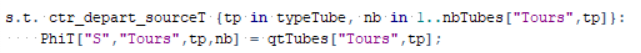
\includegraphics[width=\textwidth]{pic/source1.png}
    \caption{Contrainte de source (pour les cohortes)}
\end{figure*}

\begin{figure*}[ht]
    \centering
    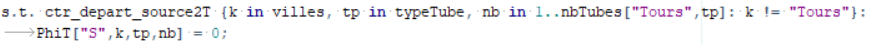
\includegraphics[width=\textwidth]{pic/source2.png}
    \caption{Contrainte de source (pour les autres villes)}
\end{figure*}

Pour chaque tube, le sommet Source envoie les quantités définies dans qtTubes pour les villes cohortes, et rien pour les autres.

\subsubsection{Contrainte de quantité max}

Elle permet de limiter le flux par rapport à la capacité max de chaque tube :

\begin{figure*}[ht]
    \centering
    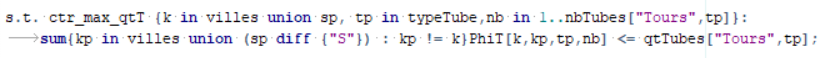
\includegraphics[width=\textwidth]{pic/maxqt.png}
    \caption{Contrainte de quantité maximum}
\end{figure*}

Pour chaque ville et chaque tube qu'elle envoie, la somme de tout ce qu'elle envoie d'un même tube ne peut pas dépasser la quantité initiale (définie dans qtTubes).  

\subsubsection{Contrainte de demande}

Elle permet de faire en sorte que la demande de chaque ville soit respectée :

\begin{figure*}[ht]
    \centering
    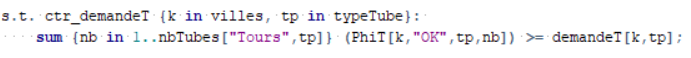
\includegraphics[width=\textwidth]{pic/demande.png}
    \caption{Contrainte de demande}
\end{figure*}

Pour chaque ville et chaque type de tube, la somme des quantités de chaque tube (du même type) envoyés au sommet OK doit être supérieure à la demande de la ville.

\subsubsection{Contrainte du puits}

Elle permet de définir la variable puits :\\ \\

\begin{figure*}[h]
    \centering
    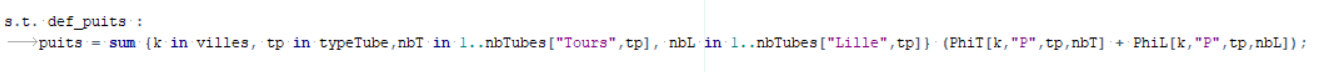
\includegraphics[width=\textwidth]{pic/puits.png}
    \caption{Contrainte du puits}
\end{figure*}

La variable puits est définie comme la somme de tout ce qu'envoie chaque ville au sommet P, tube et et type de tube confondu.

\subsubsection{Contraintes de boucles et flots}

Elles permettent de vérifier que les quantités envoyées soient égales aux quantités reçues

\begin{figure*}[ht]
    \centering
    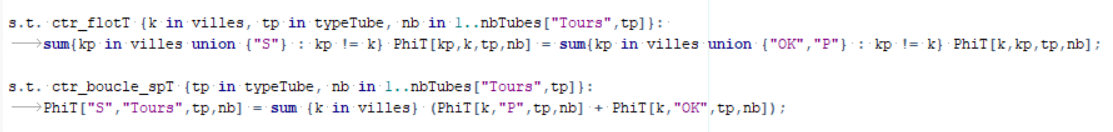
\includegraphics[width=\textwidth]{pic/flot.png}
    \caption{Contrainte de boucle et flot}
\end{figure*}

La contrainte de flot assure que pour chaque ville, la somme de ce qu'elle reçoit sur un tube est égale à la somme de ce qu'elle envoie de ce même tube.\\
La contrainte de boucle assure que pour chaque tube, la somme de ce qui est envoyé sur les sommets OK et P, toute ville confondue, est égale à la quantité initiale envoyée sur Tours. 

\subsection{Contraintes imposées}

Ces contraintes forcent le modèle à respecter les attentes réelles des centres d'analyse : 

\subsubsection{Contraintes de congélation/décongélation}

Elles permettent de d'identifier si un tube a été congelé et de compter son nombre total de cycle C/D.

\begin{figure*}[ht]
    \centering
    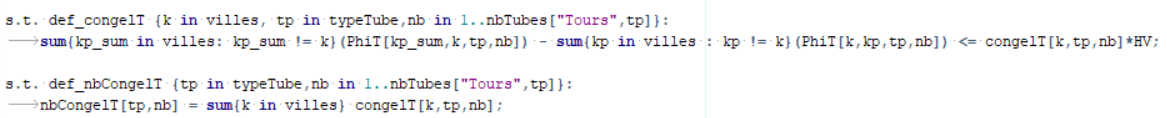
\includegraphics[width=\textwidth]{pic/congel.png}
    \caption{Contraintes de congélation/décongélation}
\end{figure*}

\paragraph{congelT}

La contrainte congelT est complexe à définir et ne prend pas en compte tous les cas de figure. Néanmoins elle fonctionne comme cela pour l'instant :\\
Pour chaque ville et chaque tube qu'elle envoie, la somme de tout ce qu'elle reçoit via d'autres villes sur ce tube \textbf{moins} la somme de tout ce qu'elle envoie aux autres villes (OK et P exclus !) depuis ce tube est inférieure ou égale à la variable de congélation de cette ville pour ce tube multiplié par HV (une très grande valeur).\\

L'idée derrière cette contrainte est si la somme de ce que la ville envoie est strictement comprise entre 0 e ce qu'elle reçoit, cela signifie que le tube a été décongelé pour pouvoir se servir, et recongelé pour envoyer le reste.
congelT étant une variable binaire, si la valeur à gauche est strictement supérieure à 0 alors congelT passera à 1 pour conserver l'égalité car 1*HV dépassera toujours le flux.

Il serait facile de définir congelT avec 2 constraintes différentes, mais la méthode de résolution de Gusek ne le permet pas (le programme tourne en boucle car valider une contrainte invalide l'autre).

\paragraph{nbCongelT}

nbCongelT est bien simple à définir car il suffit de calculer pour chaque tube combien de cycles C/D il a subi en additionnant tous les 1 de congelT pour ce tube.

\subsubsection{Contraintes d'aliquotage}

Elles permettent d'identifier si un tube a été aliquoté et de savoir en combien de tubes il a été séparé.
\begin{figure*}[ht]
    \centering
    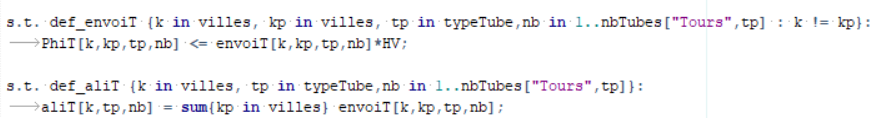
\includegraphics[width=\textwidth]{pic/aliquotage.png}
    \caption{Contraintes d'aliquotage}
\end{figure*}

\paragraph{envoiT}

envoiT est relativement simple à définir : pour chaque échange entre 2 villes différentes, si le flux est strictement positif alors envoiT est à 1, 0 sinon.

\paragraph{aliT}

De la même manière que nbCongelT, aliT compte le nombre d'envoi d'un tube depuis une même ville. A noter qu'il y a réellement \gls{aliquotage} à partir de aliT = 2.
\pagebreak

\subsection{Fonction objectif}

La fonction objectif permet de donner un but au modèle.

On identifie en premier les variables présentes dans la fonction, à ce stade là du modèle cela comprend le nombre de cycles C/D, le nombre d'aliquots et la quantité de produits jetés.

\begin{figure*}[ht]
    \centering
    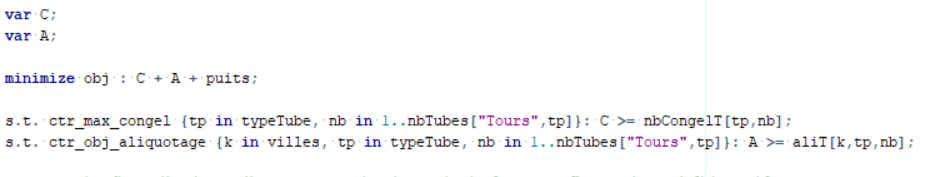
\includegraphics[width=\textwidth]{pic/objectif.png}
    \caption{Contrainte objectif}
\end{figure*}

On définit C et A respectivement comme le nombre max de cycles C/D et d'aliquots parmi tous les tubes, et on essaie de minimiser la somme des 3 variables avec le puits.\\
C'est une fonction objectif provisoire, car chaque variable est censée avoir un poids qui lui est associée pour définir un ordre de priorité. Par exemple il est peut-être plus important de limiter le nombre de cycles C/D quitte à augmenter l'\gls{aliquotage}.

\chapter{Bilan du semestre 9}

Toute la partie de prise en main du sujet et la rédaction du cahier des spécifications s'est déroulée sans accroc et même avec un peu d'avance, étant donné qu'il n'y avait pas énormément de documentation à consulter et que le système possède peu de fonctionnalités.\\
Cependant la 2ème modélisation avec la contrainte de congélation a pris plus de temps que prévu, suite à des difficultés liées à l'écriture des contraintes et la façon dont Gusek fonctionne, entraînant des retards sur le début du S10.\\
Dans l'idéal les contraintes de congélation et d'\gls{aliquotage} seront fonctionnelles avant la rentrée, afin d'enchaîner rapidement sur l'implémentation à l'aide d'un solveur.


\begin{appendix}
\selectlanguage{french}

\chapter{Planification, gestion de projet}   

\section{Evolution du projet}

Le diagramme de Gantt initial :
\begin{figure*}[ht]
    \centering
    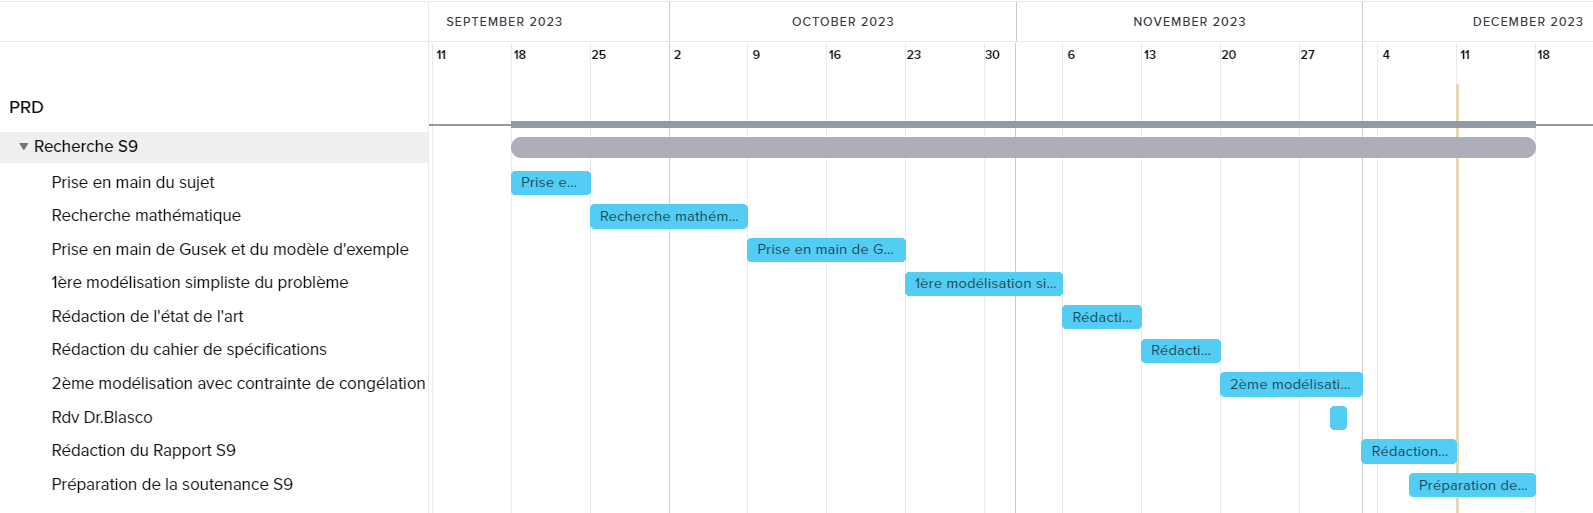
\includegraphics[width=\textwidth]{pic/gantts91.png}
    \caption{Diagramme de Gantt initial}
\end{figure*}

Le diagramme de Gantt final :
\begin{figure*}[ht]
    \centering
    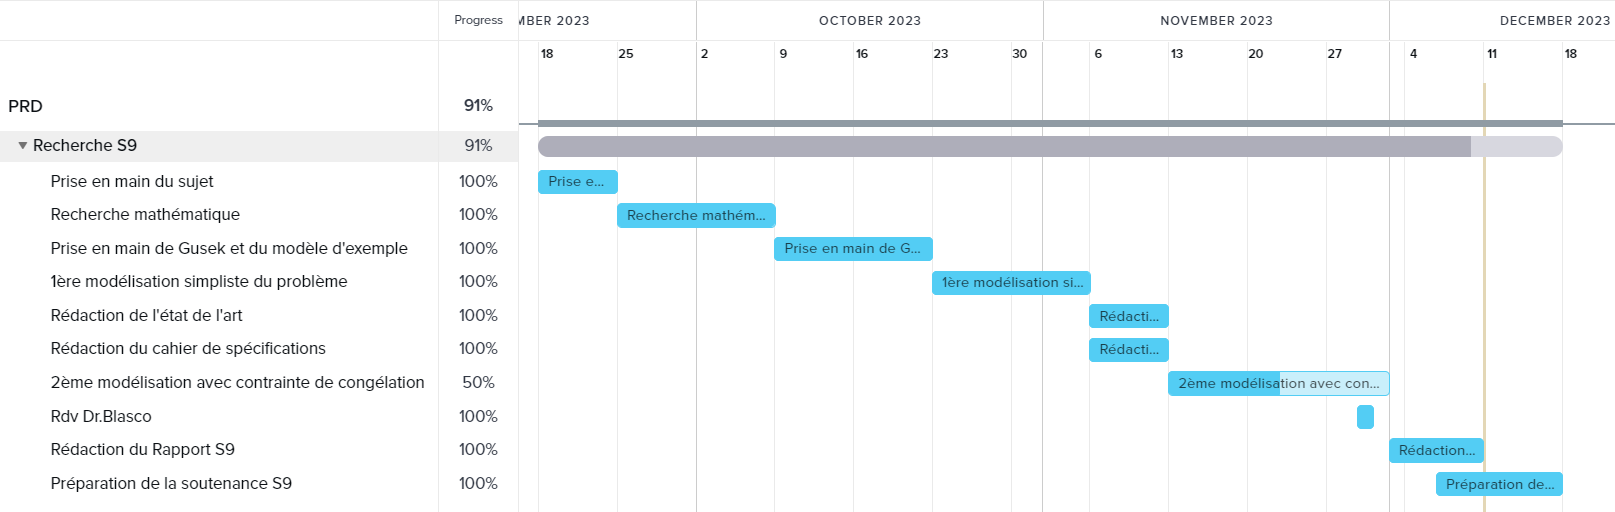
\includegraphics[width=\textwidth]{pic/gantts92.png}
    \caption{Diagramme de Gantt final}
\end{figure*}

Comme dit dans le bilan, la rédaction de l'état de l'art et du cahier de spécifications s'est avérée plus courte que prévue, ce qui m'a permis de commencer la 2ème modélisation plus tôt.\\
Malgré cela j'ai quand même pris du retard sur le S10 car je n'ai pas réussi à faire en sorte que la modélisation soit fonctionnelle avant la soutenance (elle marche dans certains cas mais il y a encore des bugs).
Dans l'ensemble j'ai plutôt bien respecté le planning initial.

\section{Description des tâches}

\paragraph{Tâche 1: Prise en main du sujet}

\begin{itemize}
    \item Date de début: 18/09/2023
    \item Date de fin: 25/09/2023
    \item Durée: 1 semaine
    \item
        Description: Lecture du sujet et des documents fournis, recherche des termes médicaux spécifiques (aliquotage...).
\end{itemize}

\paragraph{Tâche 2: Recherche mathématique}

\begin{itemize}
    \item Date de début: 25/09/2023
    \item Date de fin: 09/10/2023
    \item Durée: 2 semaines
    \item
        Description: Recherche internet des différents concepts mathématiques du sujet : Théorie des graphes, TSP, recherche opérationnelle. Renseignements sur la programmation par contraintes.
\end{itemize}

\paragraph{Tâche 3: Prise en main de Gusek et du modèle d'exemple}

\begin{itemize}
    \item Date de début: 09/10/2023
    \item Date de fin: 23/10/2023
    \item Durée: 2 semaines
    \item
        Description: Compréhension du modèle d'exemple fourni par M.Billaut : fonctionnement, variables utilisées, définition des contraintes,...\\
        Premiers tests sur Gusek avec des codes d'exemples et sur le modèle même.
        
\end{itemize}

\paragraph{Tâche 4: 1ère modélisation du problème}

\begin{itemize}
    \item Date de début: 23/10/2023
    \item Date de fin: 06/11/2023
    \item Durée: 2 semaines
    \item
        Description: Réparation des bugs présents dans le modèle initial fourni et développpement d'une première version du modèle simpliste.\\
        Discussion avec M.Billaut sur la suite du modèle.
\end{itemize}

\paragraph{Tâche 5: Rédaction de l'état de l'art}

\begin{itemize}
    \item Date de début: 06/11/2023
    \item Date de fin: 13/11/2023
    \item Durée: 1 semaine
    \item
        Description: Recherche internet sur les papiers concernant le VRP et les études dans l'organisation d'échantillons médicaux, puis rédaction de l'état de l'art.
\end{itemize}

\paragraph{Tâche 6: Rédaction du cahier de spécifications}

\begin{itemize}
    \item Date de début: 06/11/2023
    \item Date de fin: 13/11/2023
    \item Durée: 1 semaine
    \item
        Description: Rédaction du cahier de spécifications grâce à la liste des contraintes fournie en début de projet.
\end{itemize}

\paragraph{Tâche 7: 2ème modélisation avec contrainte de congélation}

\begin{itemize}
    \item Date de début: 13/11/2023
    \item Date de fin: 04/12/2023
    \item Durée: 3 semaines
    \item
        Description: Développement d'un 2ème modèle qui intègre la contrainte de congélation, en essayant d'appliquer les idées qui suivaient les réunions avec M.Billaut. Cette tâche n'a pas été terminée dans les temps.
\end{itemize}

\paragraph{Tâche 8: Rendez-vous avec Dr.Blasco}

\begin{itemize}
    \item Date de début: 29/11/2023
    \item Date de fin: 29/11/2023
    \item Durée: 1 jour
    \item
        Description: Rendez-vous avec le Dr.Blasco pour discuter du sujet, de son avancée et comparaison entre les résultats donnés par les 1ers modèles et ses attentes. Explication de l'organisation actuelle de la distribution des échantillons.  
\end{itemize}

\paragraph{Tâche 9: Rédaction du Rapport S9}

\begin{itemize}
    \item Date de début: 04/12/2023
    \item Date de fin: 10/12/2023
    \item Durée: 6 jours
    \item
        Description: Rédaction de ce rapport
\end{itemize}

\paragraph{Tâche 10: Préparation de la soutenance S9}

\begin{itemize}
    \item Date de début: 06/12/2023
    \item Date de fin: 13/12/2023
    \item Durée: 1 semaine
    \item
        Description: Création du support pour la soutenance du semestre 9 et préparation de la soutenance en elle-même. 
\end{itemize}

\chapter{Cahier de Spécifications}

\section{spécifications Fonctionnelles}
Il n'y aura que 3 fonctionnalités à développer pour ce projet, à savoir : 
\begin{itemize}
    \item Lecture des fichiers d'entrée
    \item Résolution du modèle
    \item Création des fichiers de sortie
\end{itemize}

%~ \setcounter{secnumdepth}{2}
%~ \renewcommand\thesection{\arabic{section}} 

\subsection{ Définition de la fonction 1 : Lecture des fichiers d'entrée}

\paragraph{Description de la fonction 1 :}
 
\begin{description}
    \item[Lecture du fichier d'entrée] ~ \\
        Entrée : Fichier de données contenant :
        \begin{itemize}
            \item les villes,
            \item les cohortes parmi ces villes,
            \item les types d'échantillons prélevés,
            \item pour chacune des cohortes le nombre de tubes prélevés de chaque type par patient et la quantité en mL de chacun de ces tubes. 
        \end{itemize} \\
        Sortie : Rien
        Pré-conditions : Le fichier doit être conforme (bon format, bonne nomenclature, ect...) \\
        Post-conditions : Rien
\end{description}

\subsection{Définition de la fonction 2 : Résolution du modèle}

\paragraph{Description de la fonction 2:}

\begin{description}
    \item[Variables d'entrée] ~ \\
        Entrée : Données du fichier d'entrée.\\ 
        Sortie : Variables initialisées\\
        Pré-conditions : Aucune \\
        Post-conditions : Les variables ont le bon type et la bonne dimension.

    \item[Résolution du modèle] ~ \\
        Entrée : Variables initialisées.\\ 
        Sortie : Variables du modèle après résolution\\
        Pré-conditions : Le modèle doit être solvable en temps acceptable\\
        Postconditions : Aucune
\end{description}

\subsection{Définition de la fonction 3 : Création des fichiers de sortie}

\paragraph{Description de la fonction 3:}

\begin{description}
    \item[Variables de sortie] ~ \\
        Entrée : Variables du modèle après résolution\\ 
        Sortie : Fichiers de résultats\\
        Pré-conditions : Le modèle n'a pas échoué \\
        Post-conditions : Les résultats sont écrits sur plusieurs fichiers différents, un pour chaque contrainte majeure (on écrit le contenu de chaque variable importante dans le fichier correspondant) .

    \item[Analyse des résultats] ~ \\
        Entrée : Fichiers de résultats.\\ 
        Sortie : Fichiers d'instructions à suivre et graphe correspondant à la répartition des échantillons \\
        Pré-conditions : Aucune\\
        Post-conditions : Aucune
\end{description}

\section{Spécifications non fonctionnelles}

\subsection{Contraintes de développement et conception}

Il n'y a pas d'environnement de développement imposé, mais le modèle doit répondre au mieux aux contraintes données par le Dr.Blasco.

\subsection{Contraintes de fonctionnement et d’exploitation}

\subsubsection{Performances}
Ce problème implique d'avoir beaucoup de contraintes qui se chevauchent, ce qui peut rendre le temps de résolution très long même avec une petite instance de données. Malgré tout, on peut espérer atteindre des temps avoisinant la minute.

\subsubsection{Capacités}
Comme dit plus haut le modèle aura probablement du mal à passer à l'échelle, d'autant plus que le nombre et la complexité des contraintes ne fera qu'augmenter après chaque nouvelle version, afin d'intégrer d'éventuels changements demandés par les centres d'analyses. C'est pourquoi il faudrait limiter le nombre de villes à 10, voir même moins en fonction des capacités du modèle et de mon avancée tout au long du projet. 

\subsubsection{Contrôlabilité}
Etant le seul utilisateur du système, la seule chose pouvant améliorer la contôlabilité de celui-ci serait d'ajouter un "versionning" aux modèles créés pour garder une trace et revenir sur une ancienne version si besoin.

\subsubsection{Sécurité}
Pour l'instant les données ne sont pas anonymisées et ne nécessitent pas de traitement particulier. C'est identique pour l'utilisateur, il n'y a pas encore de système de connexion prévu.                                                         

\end{appendix}

\end{document}


